\documentclass[10pt]{beamer}

\usetheme[progressbar=frametitle]{metropolis}
\usepackage{appendixnumberbeamer}

\usepackage{booktabs}
\usepackage[scale=2]{ccicons}

\usepackage{pgfplots}
\usepgfplotslibrary{dateplot}

\usepackage{xspace}
\newcommand{\themename}{\textbf{\textsc{metropolis}}\xspace}

\title{Code Generation for SPL in Rust}
\subtitle{Compiler Construction presentation}
\date{}
\author{Oussama Danba}

\begin{document}

\maketitle

\begin{frame}{Table of Contents}
  \setbeamertemplate{section in toc}[sections numbered]
  \tableofcontents[hideallsubsections]
\end{frame}

% start with a short recap
\section{General Information}
\begin{frame}{General Information}
    \begin{itemize}
        \item Recap: Monomorphic Type Checking with an exception for print and isEmpty
        \begin{itemize}
            \item Since we know the type of the arguments we can generate inline code for every specific print rather than having a true polymorphic function.
        \end{itemize}
        \item Code generator about 500 lines of code
        \item Lists and tuples are on the heap thus a variable has a pointer to the heap. Basic values are on the stack unless they are contained in a list or tuple.
    \end{itemize}
\end{frame}

% use the board here!
\section{Memory Layout}
\begin{frame}{Global Variables}
    \begin{itemize}
        \item Crucial insight: Every expression fits in one word of memory since they result in either a basic type or a pointer.
        \item We can thus store global variables in a continuous memory region either on the stack or the heap.
        \begin{itemize}
            \item I've chosen to store the global variables at the start of the stack. Since the start of the stack moves depending on how large the code segment we store the start of the stack in register R5.
        \end{itemize}
    \end{itemize}
\end{frame}

\begin{frame}{Stack Frame}
    \begin{itemize}
        \item First there are \textit{n} parameters for this function.
        \item Then there is the return address.
        \item Then there is a register that holds the previous markpointer. The new markpointer will point to this address so we can find parameters/locals relative to it.
        \item Then there are \textit{n} local variables.
    \end{itemize}
    The calling function ensures the parameters are on the stack.
    
    The function being called creates the rest of the stack. It is also responsible for cleaning up the stack, including the parameters. (It writes the return value to register RR before doing so!).
\end{frame}

\begin{frame}{Example Stack Frame}
    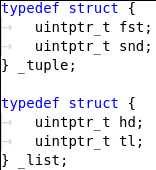
\includegraphics[width=0.7\textwidth]{presentation3/1.png}

    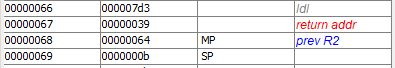
\includegraphics[width=\textwidth]{presentation3/2.png}
\end{frame}

\begin{frame}{Tuples in Heap}
    \begin{itemize}
        \item As mentioned before on the stack we have a pointer to the heap when dealing with tuples.
        \item Since tuples can only contain two items in SPL we reserve two words for the tuple in the heap. In each word a value of the tuple is stored. These values are either basic values or a pointer to another tuple/lists allowing nested tuples (and lists within tuples).
    \end{itemize}
\end{frame}

% draw on board
\begin{frame}{Lists in Heap}
    \begin{itemize}
        \item Rather than putting the list in continuous memory I opted to implement lists as linked lists in the heap. (Avoids having to copy every entry when adding a value to a list.)
        \item A pointer to a list is a pointer to two words of memory. The first word simply contains the value of that entry whereas the second word contains a pointer to the following entry of the list.
        \item The empty list is encoded by having the second word point to 0x0. Since this is guaranteed to be in the code segment we can safely use this as a marker.
        \begin{itemize}
            \item The empty list can double as a marker to mark the ending of a list since it is guaranteed to be the last entry in the list.
        \end{itemize}
    \end{itemize}
\end{frame}

\section{Code Generation}
\begin{frame}{Generating Code for Expressions 1}
    \begin{itemize}
        \item Started with the assumption that every expression results in a single value. The generated code actually makes sure this is the case!
        \item Start by implementing the literals as they simply immediately put a value on the stack with no computation.
        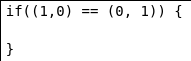
\includegraphics[width=\textwidth]{presentation3/3.png}
        \item Then slowly start expanding
    \end{itemize}
\end{frame}

\begin{frame}{Generating Code for Expressions 2}
How function calls are implemented:
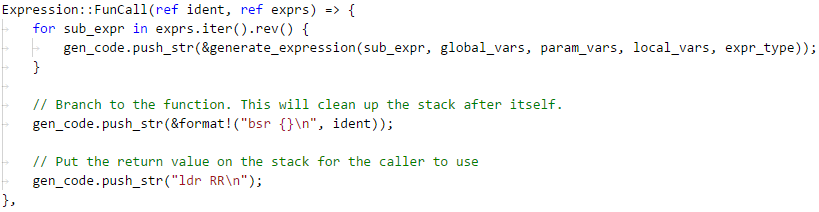
\includegraphics[width=\textwidth]{presentation3/4.png}

Once every expression is implemented we can implement global/local variables by simply storing the result of the expression at the correct place.
\end{frame}

\begin{frame}{Generating Code for Expressions 3}
    \begin{itemize}
        \item There is some trickiness such as loading the right value when using a variable identifier. If it is a global variable it must be relative to R6. Otherwise it must be relative to the markpointer (but the direction is different for parameters and locals).
        \item Another difficulty is that expressions can have runtime errors.
        \begin{itemize}
            \item What is a user asks for the head of an empty list? We can't always know at compile-time if this happens.
            \item Code is generated that checks this at runtime. It jumps to \textit{RuntimeErr} which simply halts execution. This function is user overridable (a \textbf{\textit{very primitive}} form of error handling).
        \end{itemize}
        \item Implementing ==/!= is annoying since they work for tuples and lists. Length of lists is not always known at compile time so the code has to account for that. In fact we don't have the length at all! Only option is to check equality per pair until we're done.
    \end{itemize}
\end{frame}

\begin{frame}{Generating Code for Statements 1}
Statement are now relatively simple to implement.
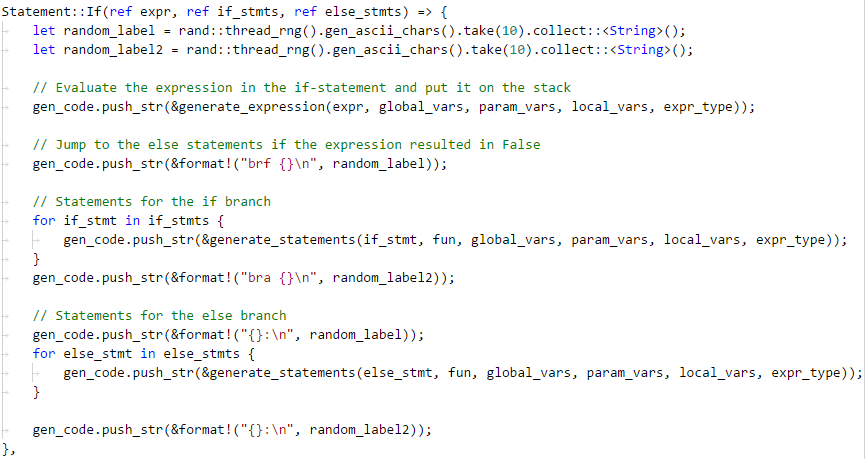
\includegraphics[width=\textwidth]{presentation3/5.png}
\end{frame}

\begin{frame}{Generating Code for Statements 2}
Some statements require a little of extra work. One such statement is return which has to store the resulting value in RR, clean up the entire stack frame, and return to the calling function.

When this is done we are able to compile programs and execute them correctly!
\end{frame}

\begin{frame}{Implementing isEmpty}
    \begin{itemize}
        \item Implementing isEmpty is actually fairly easy as the type checker ensures only lists are passed.
        \item Since lists are pointers we only have to dereference once and check if the second word is 0x0 to know if the list was empty or not!
        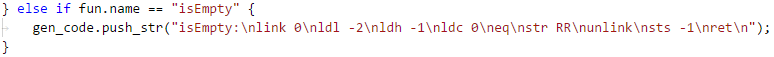
\includegraphics[width=\textwidth]{presentation3/6.png}
    \end{itemize}
\end{frame}

\begin{frame}{Implementing print}
    \begin{itemize}
        \item Idea is to implement print for basic types and then compose print for tuples/lists out of those. We know at compile time what types the tuples/lists contain so this is doable.
        \item Printing chars is easy. A simple ``trap 1'' is sufficient.
        \item Print bools is also easy. Simply check if it's True or False and print something else (this is thus simply an if/else in assembly).
        \item Printing ints? Not so easy\dots
        \begin{itemize}
            \item ``trap 0'' does what we want.
            \item However the SSM decides to put a newline at the end if you do ``trap 0'' making it unusable for this purpose. ``trap 1'' does not put a newline at the end but requires us to print the integer character per character.
        \end{itemize}
    \end{itemize}
\end{frame}

\begin{frame}{Implementing print for ints}
Idea is to do ``mod 10'' continuously and store the remainder on the stack and then divide the original number by 10. As long as the result is not done we can print another character. For convenience registers R6 and R7 are used in order to not use the stack too much. R7 stores how many characters we need to print from the stack at the end.
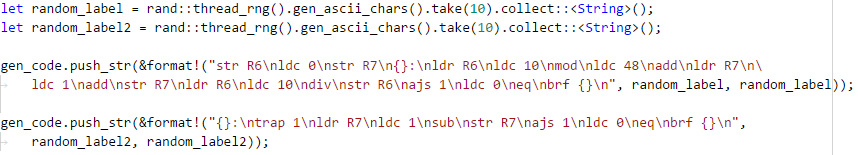
\includegraphics[width=\textwidth]{presentation3/7.png}
\end{frame}

\begin{frame}{Implementing print for tuples}
Now tuples (and lists) are fairly easy to do.
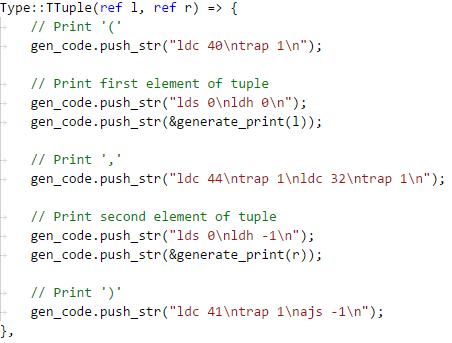
\includegraphics[width=\textwidth]{presentation3/8.png}
\end{frame}

\begin{frame}{Example of print}
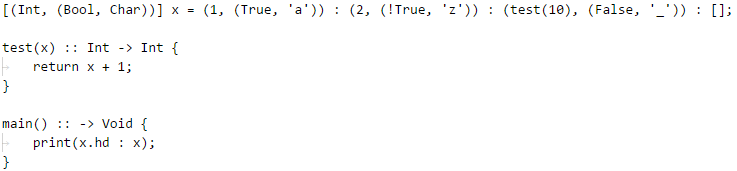
\includegraphics[width=\textwidth]{presentation3/9.png}

Produces (actually ran through SSM):\\
\texttt{(1, (True, a)) : (1, (True, a)) : (2, (False, z)) : (11, (False, \_)) : []}
\end{frame}

\section{Ending}
\begin{frame}{Afterthoughts}
    \begin{itemize}
        \item Implementing lists as linked lists ended up being more difficult than one continuous piece of memory.
        \begin{itemize}
            \item It doesn't really save in memory as we need now two words per entry instead of only one and some overhead.
            \item Is faster in cases where we're often adding new elements to a list. Probably why linked lists are often in the standard library since they have their uses.
        \end{itemize}
        \item ``trap 0'' adding a newline was annoying.
        \item Code Generator is fully functional but definitely doesn't produce optimal code (which wasn't really the purpose anyway).
    \end{itemize}
\end{frame}

{\setbeamercolor{palette primary}{fg=black, bg=yellow}
\begin{frame}[standout]
  Questions?
\end{frame}
}

\begin{frame}{License information}

  Get the source of this theme from

  \begin{center}\url{github.com/matze/mtheme}\end{center}

  The theme \emph{itself} is licensed under a
  \href{http://creativecommons.org/licenses/by-sa/4.0/}{Creative Commons
  Attribution-ShareAlike 4.0 International License}.

  \begin{center}\ccbysa\end{center}

\end{frame}

\end{document}
